\section{Application Idea}
\label{sec:application-idea}

Stockrium is proposed as a decision-support platform that helps individual investors examine Vietnamese listed companies without collecting information from many disconnected sources. The mobile application guides the user through a continuous process of discovering a stock, reviewing market and company information, configuring an analysis, receiving a multi-perspective assessment, and investigating the supporting evidence. Technical, fundamental, and news perspectives remain distinguishable so that the recommendation is presented as an explainable synthesis rather than an unexplained prediction.

The project also provides \textit{Stockrium Lab}, a web workspace in which authenticated users can run AI analyses and historical backtests, retain experiment configurations and results, revisit detailed outputs, and compare multiple experiments side by side. These information-dense views and long-running individual-security or market-universe jobs are separated from the mobile journey because they are easier to operate and inspect on a larger web interface. A curated dataset covering price and volume history, company fundamentals, and financial news with sentiment labels supports both experiences. Stockrium remains analytical rather than transactional: it does not place securities orders, transfer funds, or connect to brokerage firms. Any investment action following an analysis remains the user's responsibility.

\subsection{Stakeholders}
\label{subsec:application-stakeholders}

The proposed system considers four principal stakeholder categories. Individual investors are the primary mobile users. Authenticated Stockrium Lab users may include investors, developers, or other users who want to inspect the pipeline through controlled experiments; these roles can be held by the same person. A securities analyst contributes practical feedback, and technical teams and service providers support the data and software infrastructure.

\begin{table}[H]
    \centering
    \caption{Principal stakeholders of Stockrium}
    \label{tab:stockrium-stakeholders}
    \small
    \begin{tabularx}{\textwidth}{>{\raggedright\arraybackslash}p{3.8cm} X}
        \toprule
        \textbf{Stakeholder} & \textbf{Description} \\
        \midrule
        Individual investors & Explore Vietnamese stocks and receive configurable, explainable analysis through the mobile application. \\
        Authenticated Stockrium Lab users & Run, retain, review, export, and compare supported AI analysis and backtesting experiments through the web workspace. \\
        Securities analyst & Assesses the system's practical usefulness and provides professional feedback. \\
        Technical teams and service providers & Develop and operate the platform or supply its data and infrastructure services. \\
        \bottomrule
    \end{tabularx}
\end{table}

\subsection{Use Case Model}
\label{subsec:application-use-cases}

Stockrium has three direct user roles. A guest accesses registration, sign-in, and account-recovery functions; an authenticated investor uses personalized exploration, analysis, and chatbot features through the mobile application; and an authenticated Stockrium Lab user runs and compares experiments through the web workspace. Figure~\ref{fig:stockrium-mobile-use-case-model} presents the guest and authenticated-investor use cases in the mobile application, while Figure~\ref{fig:stockrium-web-use-case-model} presents the Stockrium Lab use cases.

\begin{figure}[H]
    \centering
    \IfFileExists{figures/chapter3/stockrium_use_case_model_stockrium.png}{%
        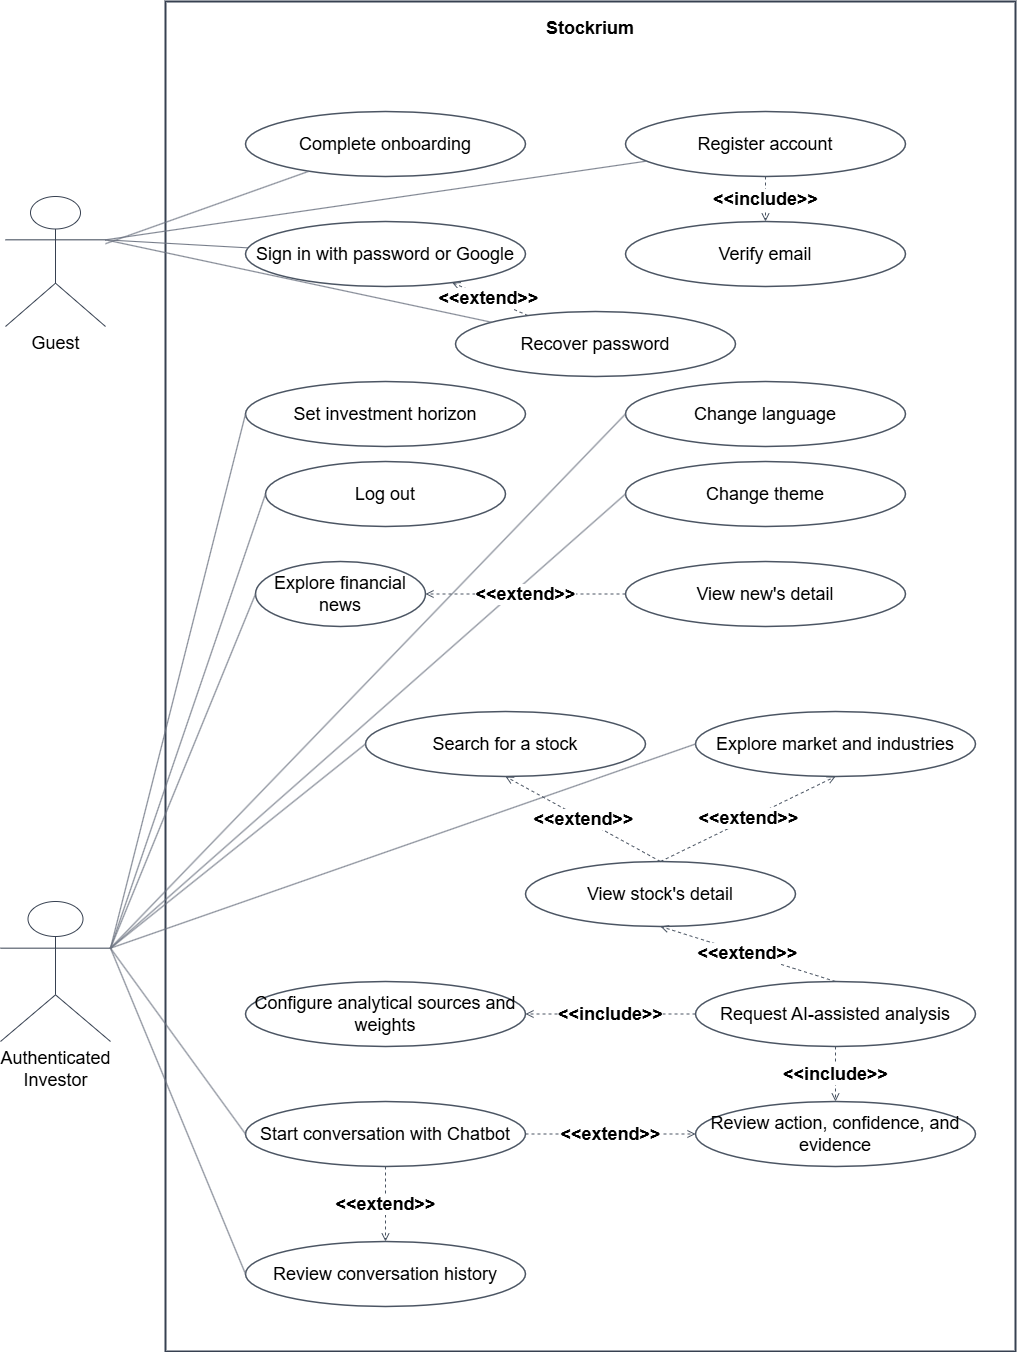
\includegraphics[width=\textwidth,height=0.8\textheight,keepaspectratio]{figures/chapter3/stockrium_use_case_model_stockrium.png}%
    }{%
        \fbox{\parbox[c][4.5cm][c]{0.92\textwidth}{\centering
        Missing figure:\\
        \texttt{figures/chapter3/stockrium\_use\_case\_model\_stockrium.png}}}%
    }
    \caption{Use-case model of the Stockrium mobile application}
    \label{fig:stockrium-mobile-use-case-model}
\end{figure}

\begin{figure}[H]
    \centering
    \IfFileExists{figures/chapter3/stockrium_use_case_model_web.png}{%
        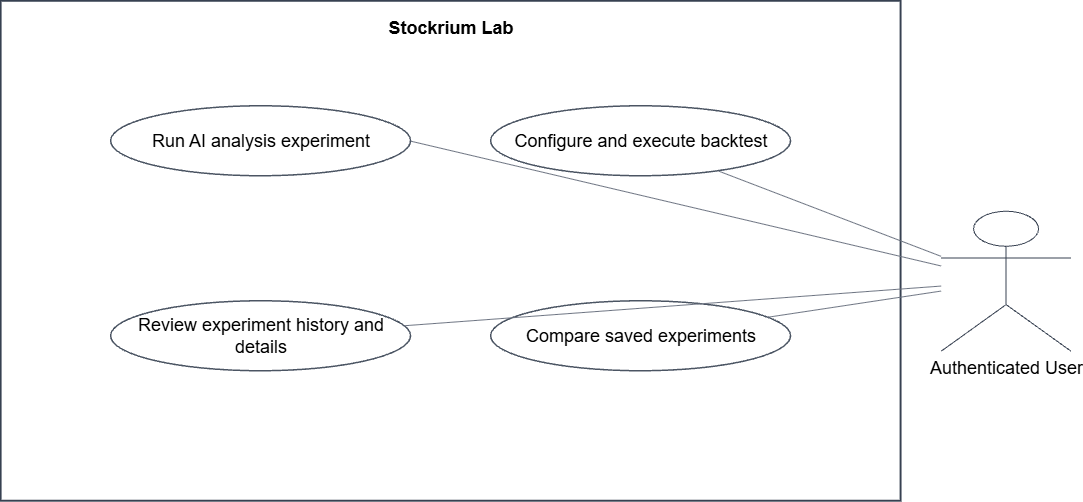
\includegraphics[width=\textwidth,height=0.8\textheight,keepaspectratio]{figures/chapter3/stockrium_use_case_model_web.png}%
    }{%
        \fbox{\parbox[c][4.5cm][c]{0.92\textwidth}{\centering
        Missing figure:\\
        \texttt{figures/chapter3/stockrium\_use\_case\_model\_web.png}}}%
    }
    \caption{Use-case model of Stockrium Lab}
    \label{fig:stockrium-web-use-case-model}
\end{figure}

{\small
\setlength\LTleft{\fill}
\setlength\LTright{\fill}
\begin{longtable}{>{\raggedright\arraybackslash}m{5.1cm} >{\raggedright\arraybackslash}m{8.7cm}}
    \caption{Use cases in the Stockrium mobile and experimentation interfaces}
    \label{tab:stockrium-use-cases} \\
    \toprule
    \textbf{Use case} & \textbf{Description} \\
    \midrule
    \endfirsthead
    \multicolumn{2}{l}{\small\itshape Table~\ref{tab:stockrium-use-cases} continued} \\
    \toprule
    \textbf{Use case} & \textbf{Description} \\
    \midrule
    \endhead
    \bottomrule
    \endfoot
    \multicolumn{2}{l}{\textbf{Mobile application}} \\
    Register account & Creates a new investor account and includes email verification. \\
    Verify email & Confirms ownership of the email address used to register the account. \\
    Sign in with password or Google & Authenticates the user through a supported sign-in method. \\
    Recover password & Restores access to an account with a forgotten password. \\
    Personalize & Adapts the application experience to the authenticated investor's preferences. \\
    Log out & Ends the current authenticated session. \\
    Explore financial news & Browses available financial articles. \\
    View news details & Opens the content and metadata of a selected financial article. \\
    Search for a stock & Finds a security by its symbol or company information. \\
    Explore market and industries & Reviews market conditions and industry groups. \\
    View stock details & Opens market, company, fundamental, technical, and news information for a selected stock. \\
    View AI-assisted analysis & Displays the AI-assisted assessment associated with the selected stock. \\
    Start conversation with Chatbot & Begins a conversational financial-support session. \\
    Review conversation history & Reopens previous chatbot sessions and messages. \\
    \midrule
    \multicolumn{2}{l}{\textbf{Stockrium Lab web workspace}} \\
    Run AI analysis experiment & Executes a supported analysis for one stock, VN30, or VN100 and stores the run as a user-owned experiment. \\
    Configure and execute backtest & Runs a supported historical simulation for one stock or VN30 and tracks its experiment status. \\
    Review experiment history and details & Filters previous experiments and opens their configuration, status, summary, detailed result, visualizations, and available reproducibility metadata. \\
    Compare saved experiments & Selects two to five experiments of the same type and compares their configurations and results side by side. \\
\end{longtable}
}

Market-data providers, news services, and language-model services are supporting dependencies rather than direct actors because they do not initiate the user goals shown in the model. Their interactions with Stockrium are described in the system architecture and data-pipeline sections of Chapter 4.

\subsection{Main Application Flows}
\label{subsec:main-application-flows}

The use cases form two primary experiences: an investor-facing mobile journey and the Stockrium Lab experimentation workflow. These flows describe user-visible behavior and intentionally treat the underlying multi-agent workflow as a single analytical service; its agents, state, and execution logic are presented in Chapter 4.

\subsubsection{Mobile Exploration and Stock-Analysis Flow}

A guest first completes onboarding and authenticates through registration, password sign-in, or the supported Google Sign-In flow. After authentication, the investor can enter a stock context from the market overview, search, financial news, or the watchlist. The stock-detail view consolidates price and volume charts, company information, fundamental data, technical indicators, and related news, allowing the investor to examine the available evidence before requesting an assessment.

The user may proceed with an automatic analysis configuration or manually select the evidence sources and their relative weights. The request combines the selected configuration, stock symbol, and saved investment horizon. Figure~\ref{fig:stockrium-primary-flow} summarizes the first part of the mobile journey, from account access and stock discovery to submission of the analysis request.

\begin{figure}[H]
    \centering
    \IfFileExists{figures/chapter3/mobile_decision_support_flow_part1.png}{%
        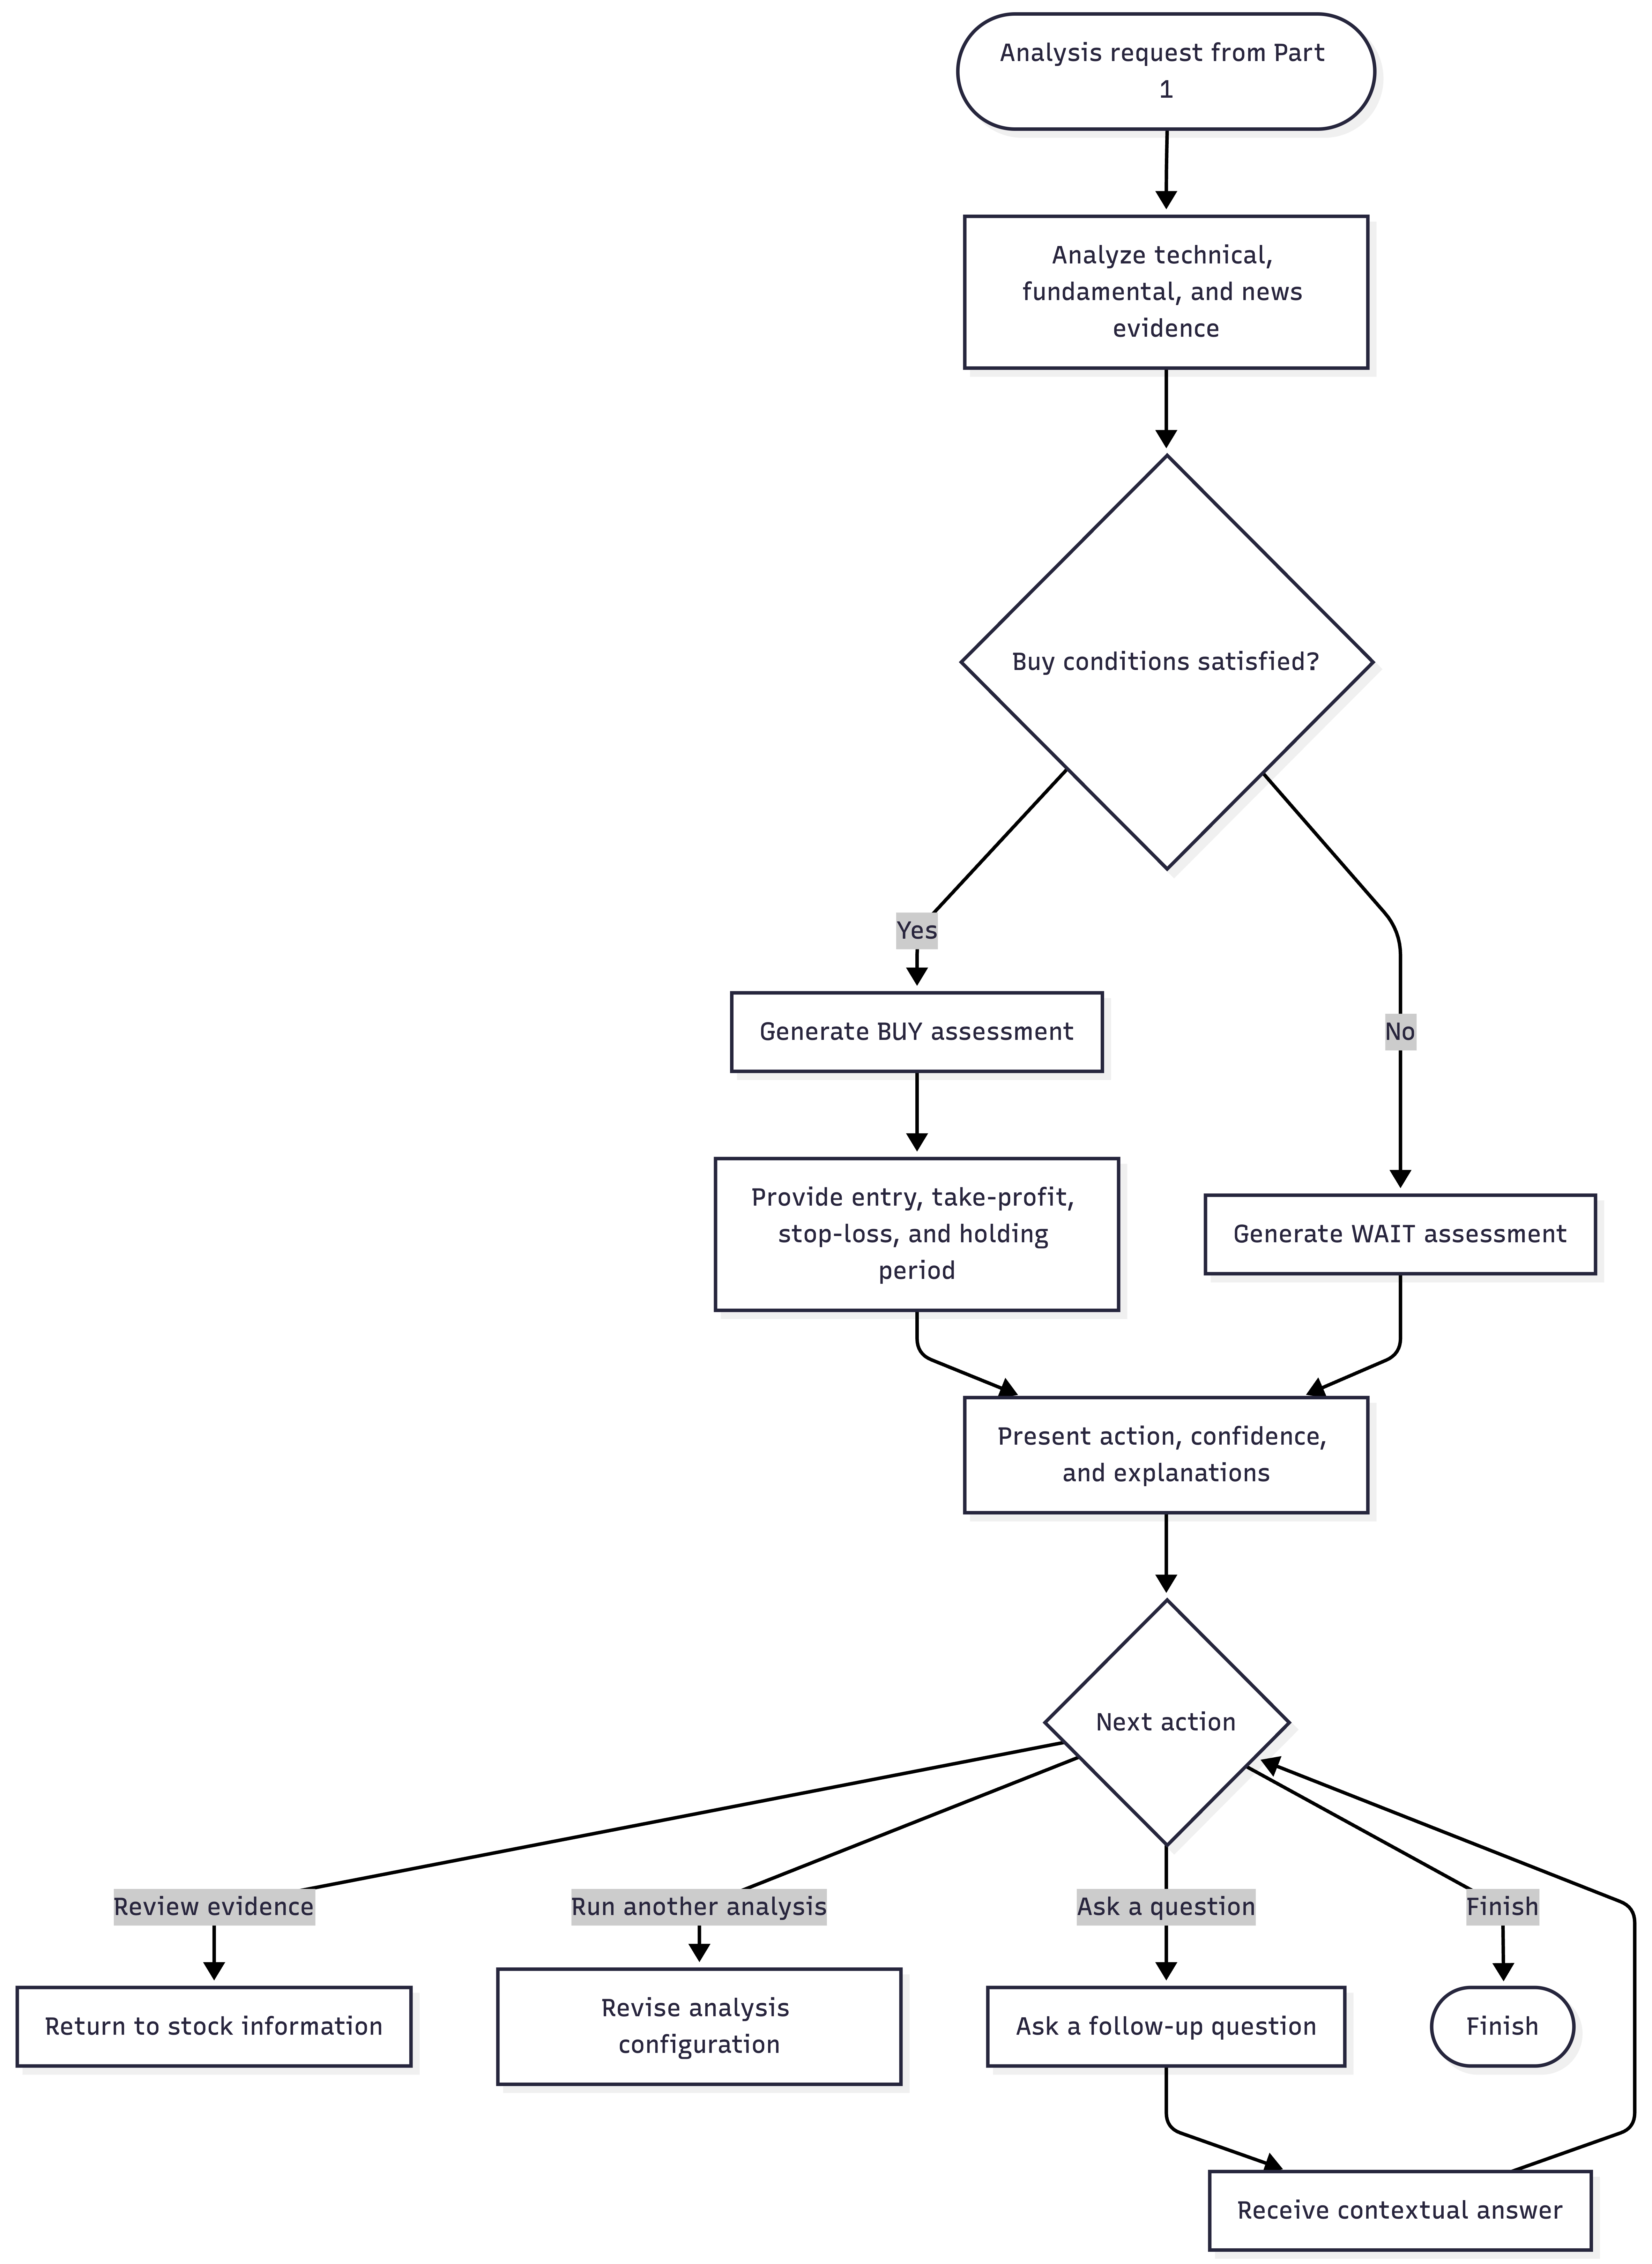
\includegraphics[width=\textwidth,height=\textheight,keepaspectratio]{figures/chapter3/mobile_decision_support_flow_part1.png}%
    }{%
        \fbox{\parbox[c][4.5cm][c]{0.92\textwidth}{\centering
        Export the Mermaid diagram as\\
        \texttt{figures/chapter3/mobile\_decision\_support\_flow\_part1.png}}}%
    }
    \caption{Mobile decision-support flow: account access, stock discovery, and analysis configuration}
    \label{fig:stockrium-primary-flow}
\end{figure}

After submission, Stockrium processes the enabled technical, fundamental, and news perspectives and returns either a \textit{Buy} or \textit{Wait} assessment. The result includes confidence and source-specific explanations; an accepted \textit{Buy} assessment may additionally contain an entry price, take-profit price, stop-loss price, and maximum holding period. Figure~\ref{fig:stockrium-analysis-result-flow} presents the second part of the journey, including evidence evaluation, recommendation validation, and subsequent user choices.

\begin{figure}[H]
    \centering
    \IfFileExists{figures/chapter3/mobile_decision_support_flow_part2.png}{%
        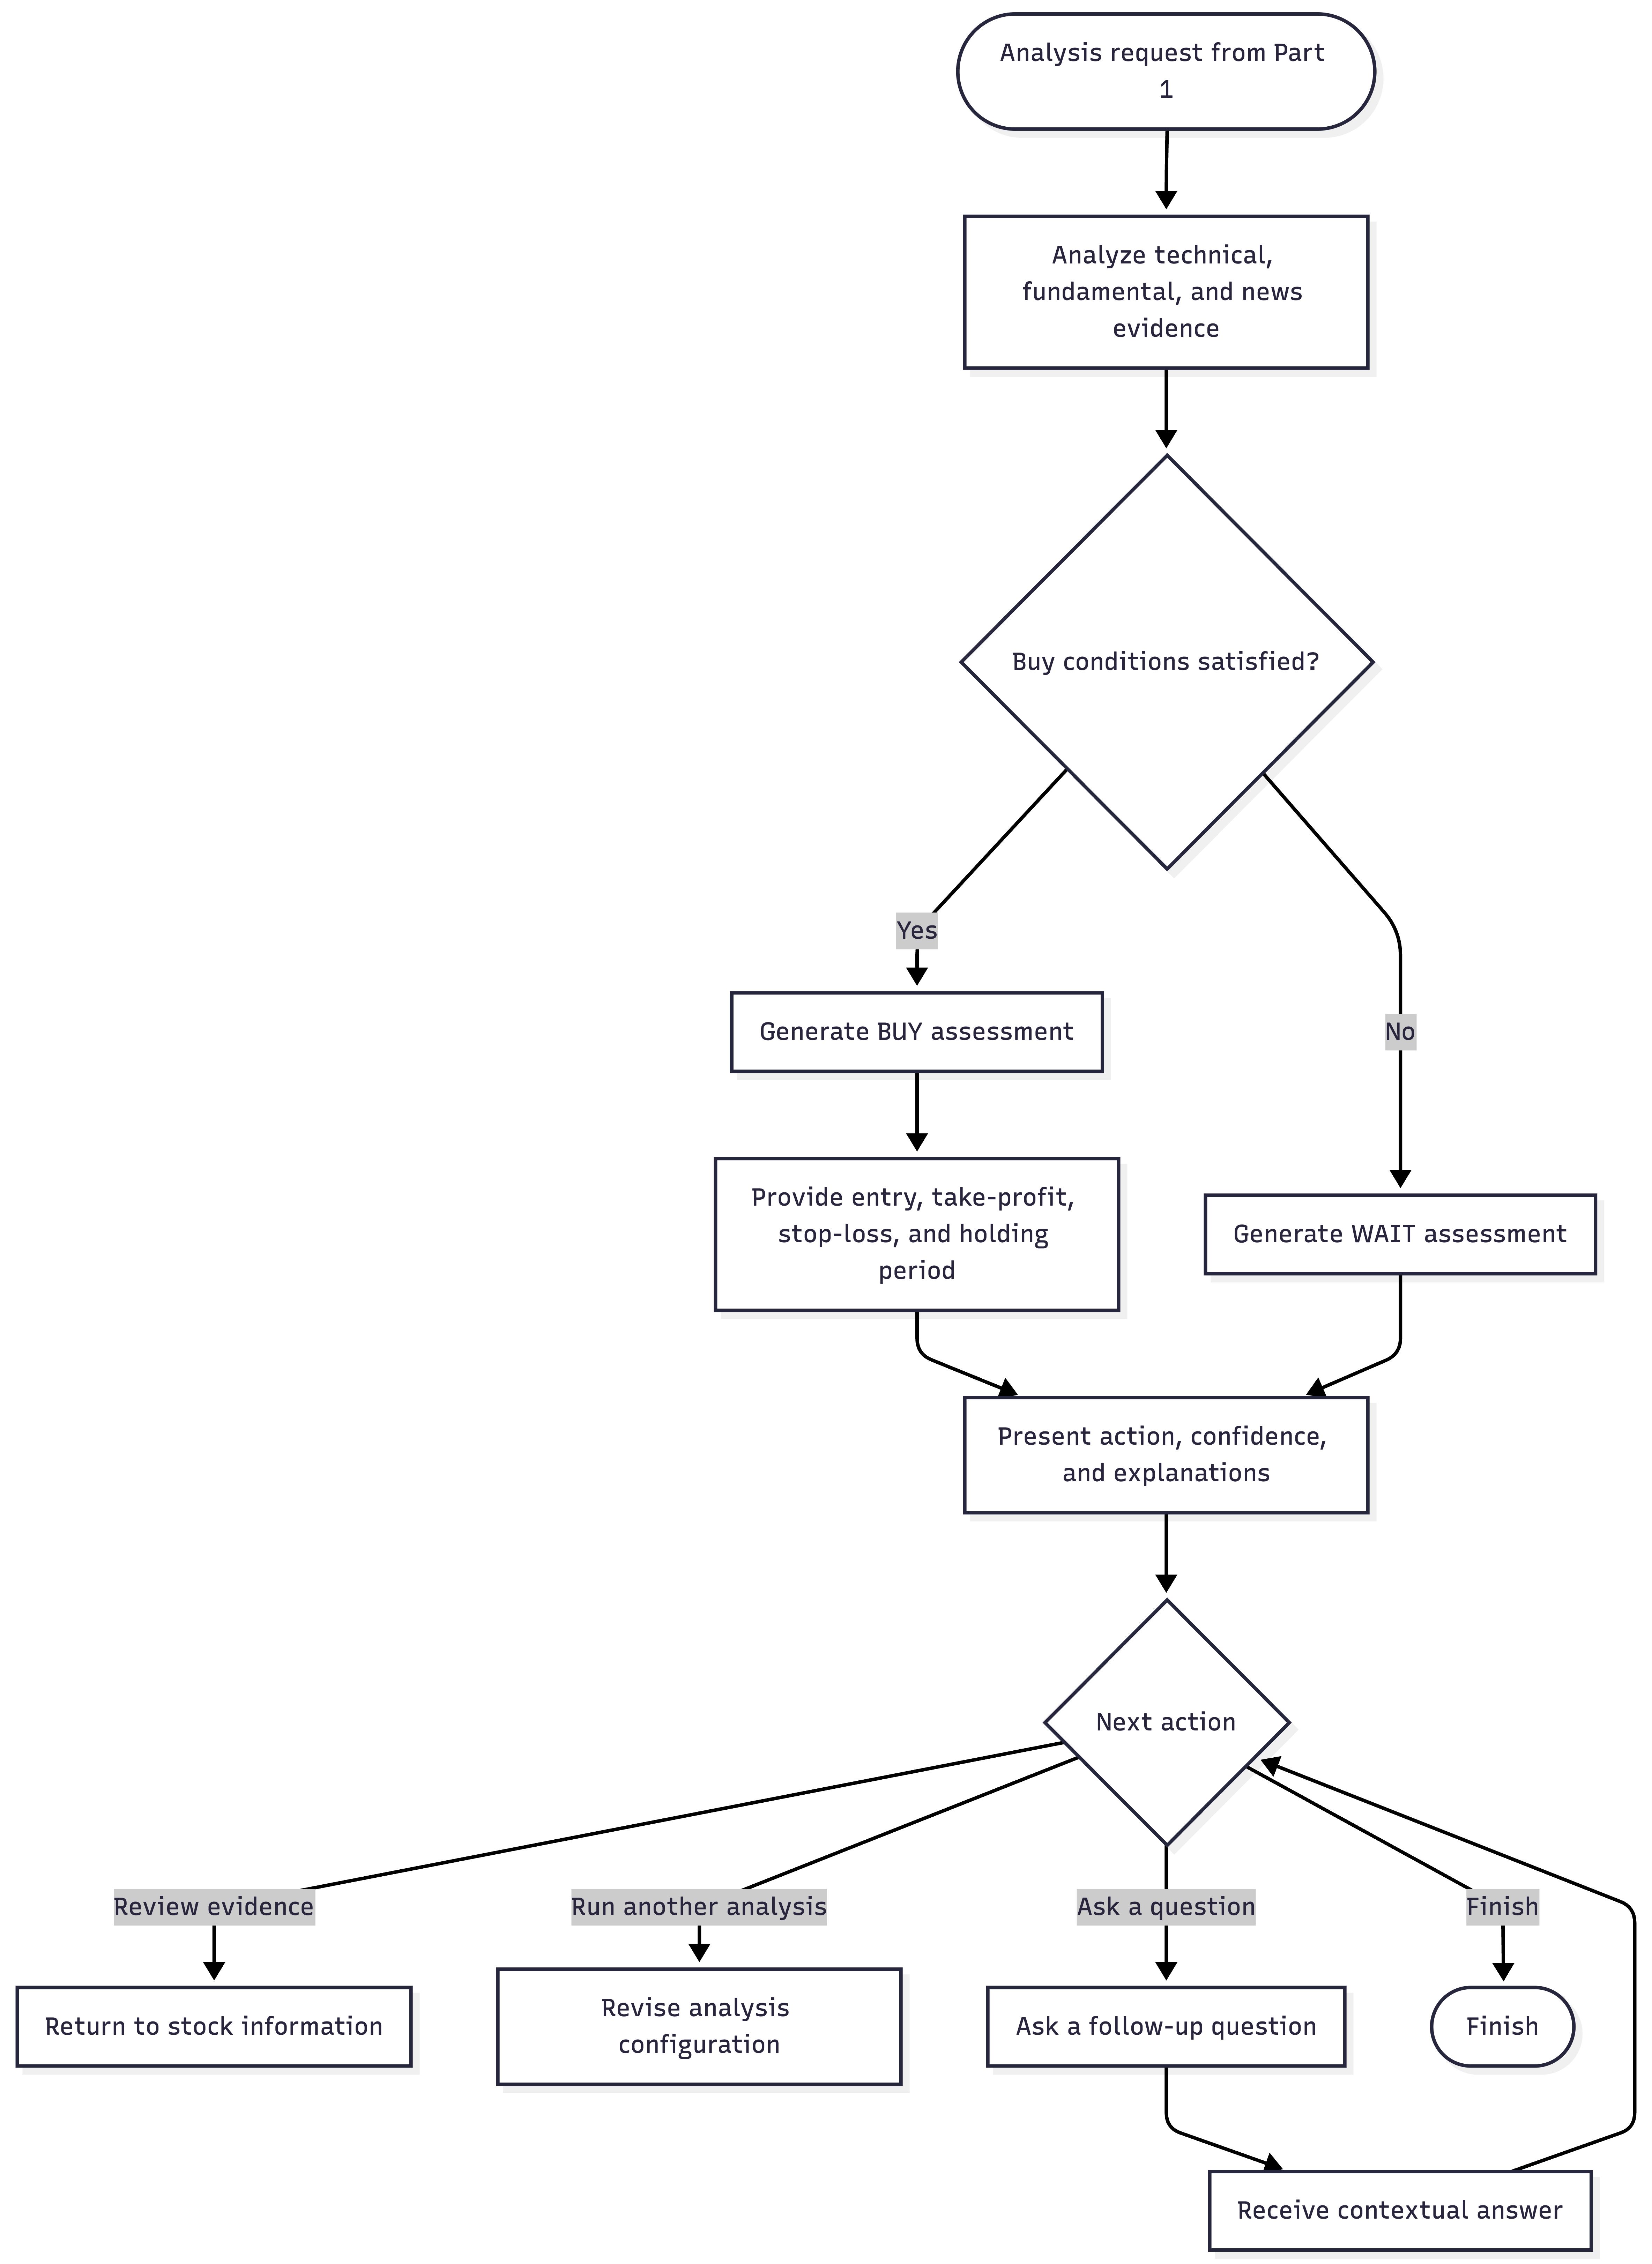
\includegraphics[width=\textwidth,height=\textheight,keepaspectratio]{figures/chapter3/mobile_decision_support_flow_part2.png}%
    }{%
        \fbox{\parbox[c][4.5cm][c]{0.92\textwidth}{\centering
        Export the Mermaid diagram as\\
        \texttt{figures/chapter3/mobile\_decision\_support\_flow\_part2.png}}}%
    }
    \caption{Mobile decision-support flow: analysis processing and recommendation}
    \label{fig:stockrium-analysis-result-flow}
\end{figure}

After reviewing the recommendation, the investor can return to the supporting charts and company data, revise the configuration, or update the watchlist. These paths form an iterative cycle in which the user continues to examine the evidence rather than acting solely on the generated action label.

\subsubsection{Stockrium Lab Experimentation and Comparison Flow}

An authenticated user opens Stockrium Lab to create a new experiment or revisit previous runs. AI-assisted analysis can be requested for an individual stock or the VN30 or VN100 universe. Backtesting can be executed for an individual stock or sequentially for the VN30 universe. The user names the experiment, selects the supported configuration, and submits it through the protected backend. Analysis results are returned after processing, whereas a backtest is accepted as a background job and can be monitored through its experiment status. Each run retains its configuration, summary, detailed output, and available reproducibility metadata under the current user's account.

The history view allows the user to filter experiments, reopen an analysis result, or load a completed backtest with its price chart, generated entries and exits, performance and risk measures, and comparison references. The user may also select from two to five experiments of the same type and compare their targets, inputs, pipeline metadata, and results side by side. This comparison is intended to expose configuration differences and pipeline behavior; a highlighted metric is not evidence that one experiment will remain superior in future market conditions. Figure~\ref{fig:stockrium-experimentation-flow} shows how execution, history review, and comparison return to the same Stockrium Lab workspace.

\begin{figure}[H]
    \centering
    \IfFileExists{figures/chapter3/experimentation_backtesting_flow.png}{%
        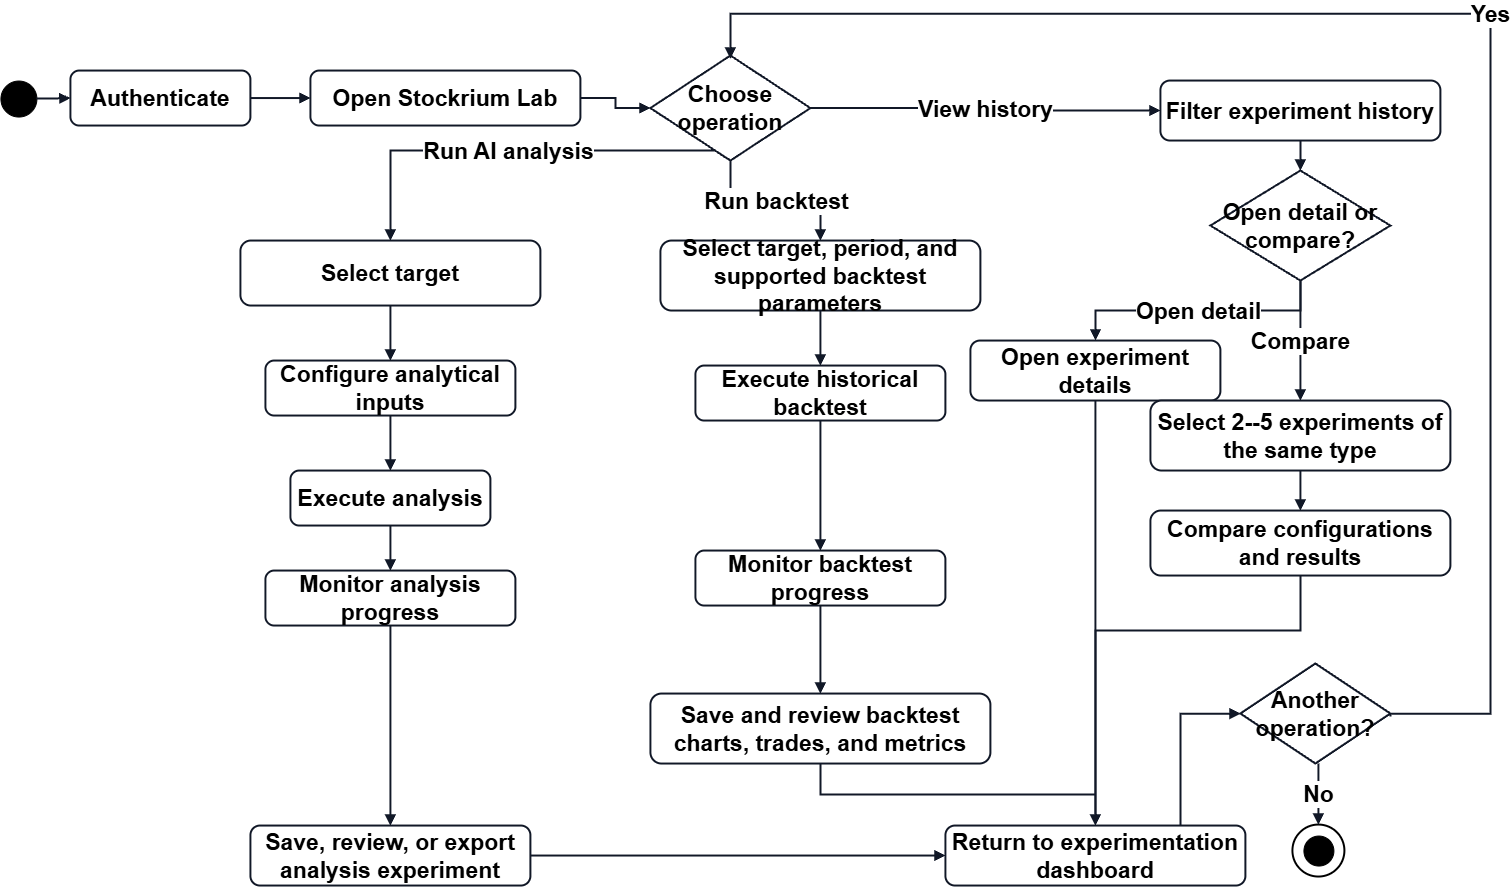
\includegraphics[width=\textwidth,height=\textheight,keepaspectratio]{figures/chapter3/experimentation_backtesting_flow.png}%
    }{%
        \fbox{\parbox[c][4.2cm][c]{0.92\textwidth}{\centering
        Export the Mermaid diagram as\\
        \texttt{figures/chapter3/experimentation\_backtesting\_flow.png}}}%
    }
    \caption{Stockrium Lab experimentation, history, and comparison flow}
    \label{fig:stockrium-experimentation-flow}
\end{figure}

The Stockrium Lab workflow supports controlled analysis, backtesting, history review, export, and experiment comparison. It is not a web trading platform and does not cause any real-market transaction. Together with the mobile journey, it positions Stockrium as an evidence-centered application and an inspectable environment in which users can test and compare the supported analytical pipeline without treating historical outcomes as guaranteed investment performance.
